\chapter{Memoria de trabajo}
Mi trabajo se ha centrado en mejorar la herramienta en los aspectos gráficos y funcionales, y añadiendo en la medida de lo posible todas las funcionalidades que hemos considerado necesarias para la aplicación.

A continuación se describen con detalles los principales cambios y mejoras que se han implementado con respecto a la versión anterior.
%%%%%%%%%%%%%%%%
\section{Diseño}
\begin{figure}[H]
    \centering
    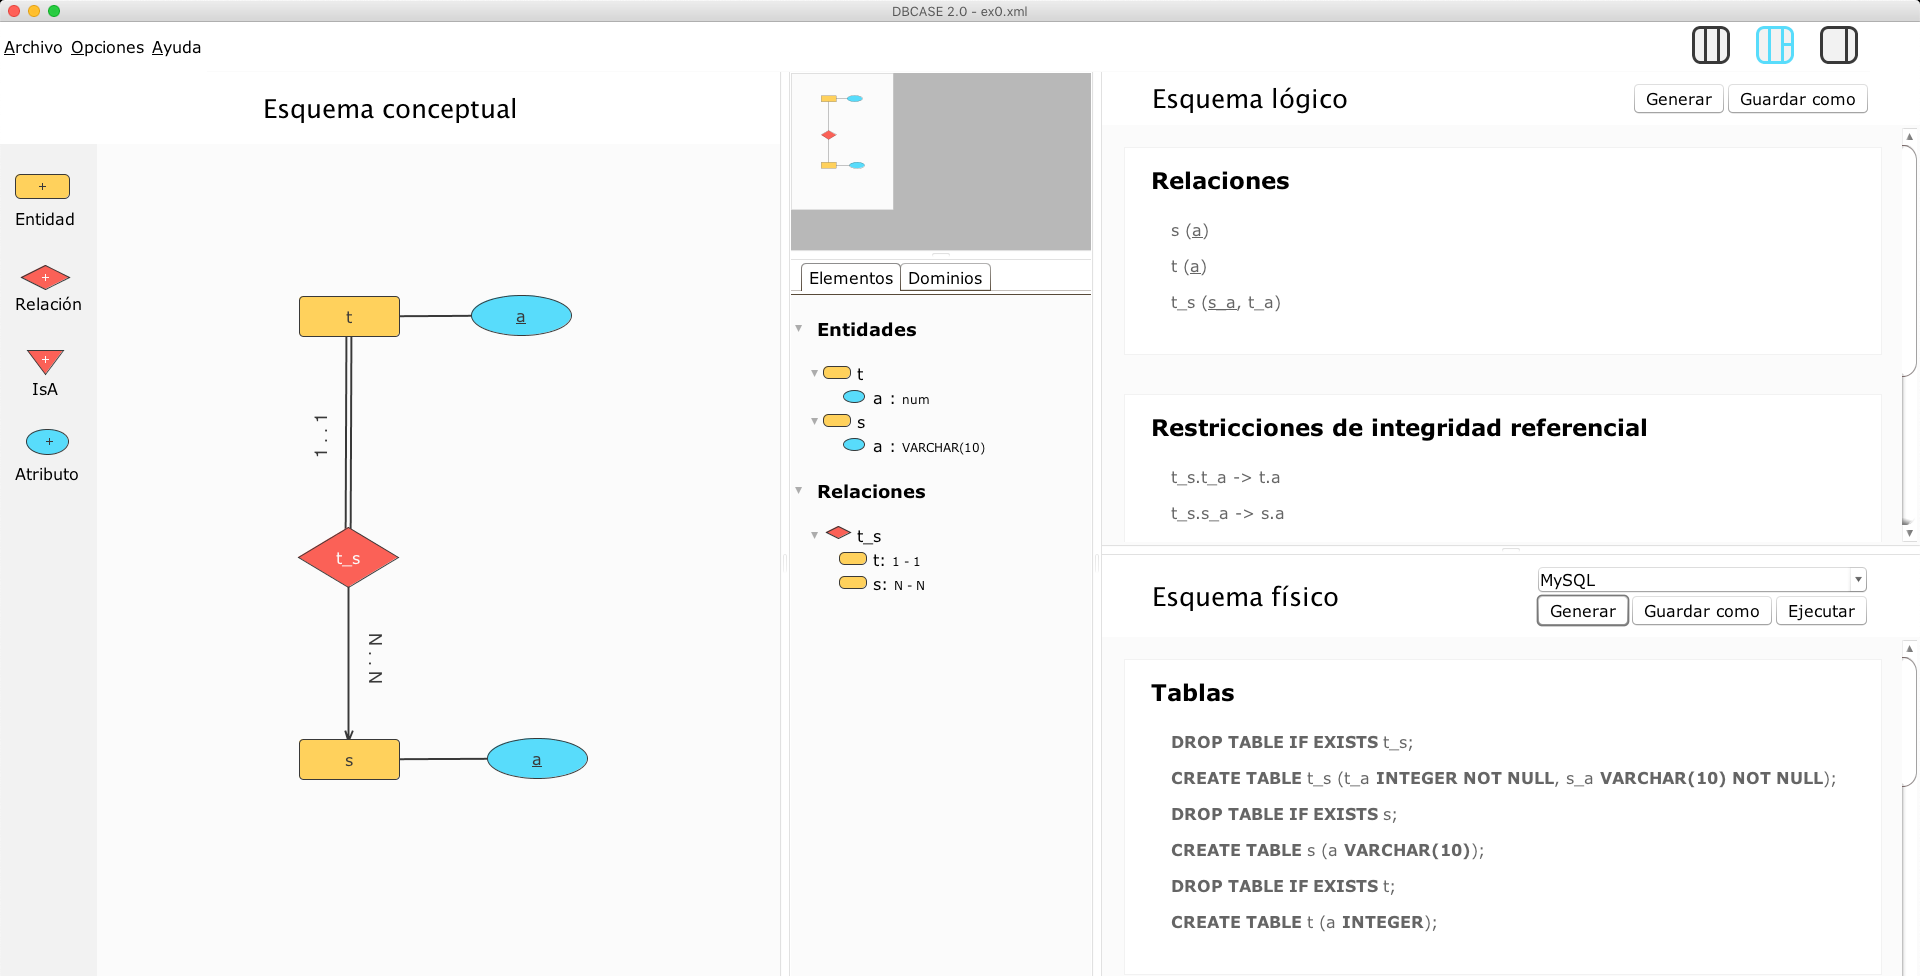
\includegraphics[width=\textwidth]{img/GUI_DBCASE.png}
    \caption{GUI de DBCASE 2.0}
\end{figure}
La aplicación ha sufrido un profundo cambio de diseño. Se ha buscado dar un aspecto más moderno a la aplicación, de forma que se han conservado las librerías gráficas con las que implementó y se ha intentado exprimir al máximo sus posibilidades.\\

\subsection{Look and Feel}
Debido a la decisión de continuar usando las librerías de java swing, se investigaron las posibilidades que ofrecía para personalizar el diseño de la interfaz. Una de las principales opciones que ofrece java swing es la de poder editar fácilmente el estilo de los paneles mediante el denominado look and feel.

\begin{lstlisting}[backgroundcolor = \color{white},
                   xleftmargin = 2cm,language=java,basicstyle=\medium]
javax.swing.UIManager.setLookAndFeel();
\end{lstlisting}

El look and feel en java swing permite cambiar el aspecto por defecto de todos los componentes visuales generados por la librería (JPanel, JFileChooser, JFrame, etc).

\subsubsection{Nimbus Look and Feel}
Java ofrece por defecto varios look and feel con los que el programador puede editar sus interfaces.\\

De las distintas opciones se decidió utilizar Nimbus Look and Feel.
\begin{quote}
    \textit{"Nimbus es un pulido Look and Feel multiplataforma introducido en Java SE 6 Update 10 (6u10)."}\cite{nimbus}
\end{quote}

Entre los principales motivos que llevaron a tomar esta decisión destacan:
\begin{itemize}
    \item Su aspecto moderno y redondeado suponía un importante lavado de cara con respecto al aspecto anterior, y era una cualidad diferencial con respecto a las otras opciones.
    \item El hecho de que sea multiplataforma permite que la aplicación tenga un aspecto uniforme en los distintos sistemas operativos.
    \item La capacidad de personalización, que permite elegir el aspecto de prácticamente cualquier elemento visual de la interfaz.
\end{itemize}
\subsubsection{Nimbus Look and Feel personalizado}
La personalización de Nimbus se ha centrado principalmente en dos aspectos.
\begin{itemize}
    \item La fuente de texto: se ha buscado que la aplicación sea lo más accesible y clara posible, por lo que se ha utilizado la fuente \textbf{Verdana 16}, por ser una de las más usadas y simples, y a tamaño 16 para que la lectura por parte del usuario se realice sin dificultades.
    \item Los colores de los elementos, paneles, botones y menús. De forma que permitiera la implementación de distintos temas.
\end{itemize}

\subsection{Temas}
Un aspecto en el que se ha centrado el trabajo ha sido en la implementación de temas que permitieran al usuario personalizar la interfaz gráfica.\\

Los dos objetivos que se perseguían con la implementación de temas eran:
\begin{itemize}
    \item Habilitar un tema oscuro, tan usado en las interfaces de usuario modernas, que permite reducir la fatiga visual y hace más cómodo el trabajo en entornos con poca luz.
    \item Permitir a los usuarios crear y personalizar sus propios temas, pudiendo escoger los colores principales que utiliza la aplicación.
\end{itemize}
\subsubsection{Detalles de la implementación de los temas}
Para que la creación y personalización de temas fuera lo más dinámica posible se decidió que los distintos temas se almacenasen en archivos \textbf{json}\cite{json}, externos al programa, de forma que el usuario pueda modificarlos, copiarlos o eliminarlos fácilmente. Los archivos json que contienen los temas se almacenan en la carpeta "themes".\\

\begin{quote}
\textit{"JSON (acrónimo de JavaScript Object Notation) es un formato de texto sencillo para el intercambio de datos."}
\end{quote}

Dentro del archivo json, se establecen el nombre del tema, y los colores de los principales elementos de la aplicación, entre ellos algunos de los más destacables son:
\begin{itemize}
    \item El color de los elementos del diagrama (relaciones, atributos y entidades).
    \item El color de fondo del diagrama.
    \item El color principal de la aplicación (utilizado por Nimbus para pintar el fondo de los paneles, botones, etc).
    \item El color de las fuentes, tanto de la fuente de los paneles como de la fuente de los cuadros de texto de los esquemas relacional y físico.
\end{itemize}

Dentro del menú de opciones, el usuario tiene la posibilidad de elegir un tema de entre todos los temas disponibles dentro de la carpeta "themes".\\

Se han incorporado dos temas con la aplicación:
\begin{itemize}
    \item \textbf{Light} o tema claro: es el tema por defecto. Utiliza colores blancos y grises para la aplicación, y colores elementales para resaltar los elementos del diagrama.
    \item \textbf{Dark} o tema oscuro: tiñe la interfaz con colores negros manteniendo el protagonismo de los elementos del diagrama.
\end{itemize}

Además el usuario puede crear sus propios temas añadiendo un archivo en formato json a la carpeta "themes" que siga la estructura de los temas incorporados.\\

Para el manejo interno de los temas se ha creado una clase theme utilizando el patrón de diseño \textbf{"Singleton"}\cite{singleton}, lo que permite a cualquier otra clase obtener una instancia de la misma y poder consultar en ella los colores de forma sencilla.

\subsection{Disposición de paneles}
Uno de los mayores cambios que ha sufrido la interfaz de usuario ha sido la disposición de los distintos paneles. Se ha buscado una GUI más clara y sencilla sin perder ninguna de las funcionalidades.\\

Con respecto a la versión anterior, los cambios principales que ha sufrido la interfaz son:
\begin{itemize}
    \item Se ha pasado de una interfaz dividida en dos pestañas (diagrama entidad-relación y generación de código) a una sola, de forma que ahora se puede ver de un vistazo el diagrama y el código generado.
    \item El panel de generación de código se ha dividido en dos paneles distintos: Esquema lógico y esquema físico. De esta manera quedan ambos lenguajes en paneles independientes.
    \item Se han unificado el panel de información y el panel de dominios en un solo JTabbedPane.
    \item Los paneles están separados mediante la clase JSplitPane \cite{split}, lo que permite al usuario cambiar a su antojo el tamaño de cada panel.
    \item Se ha eliminado el panel de sucesos, ya que su utilidad era más bien para el desarrollo de la aplicación y no para el usuario.
\end{itemize}
\subsection{Panel de información}

\begin{figure}[H]
    \centering
    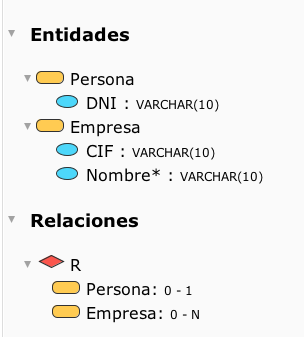
\includegraphics[width=0.4\textwidth]{img/PanelInfo.png}
    \caption{Panel de Información}
\end{figure}

El panel de información muestra un esquema en forma de árbol del modelo entidad relación existente en el panel de diseño, y en él se puede ver de forma esquemática todos los elementos y cómo están relacionados.\\

El panel de información ha sufrido profundos cambios que se describen a continuación:

\begin{itemize}
    \item Ahora el panel muestra en todo momento la información global de todo el esquema creado por el usuario, al contrario que en la versión anterior, en la que solo mostraba la información de los elementos seleccionados.
    \item El panel de información ha pasado a dividirse en dos sectores: entidades y relaciones.
    \begin{itemize}
        \item \textbf{Entidades}: muestra todas las entidades del esquema y sus atributos. Muestra el dominio del atributo al lado del nombre y representa gráficamente de forma correcta los subatributos de atributos compuestos (como ramas de los mismos).
        \item \textbf{Relaciones}: muestra todas las relaciones del esquema y para cada una de ellas muestra sus atributos y las entidades que relaciona. Para cada una de las entidades muestra la cardinalidad al lado del nombre.\\
        
        Para las relaciones ISA muestra la entidad padre como la primera entidad de la relación, y las entidades hijas con un icono que las diferencia como tal.
    \end{itemize}
    \item Para la renderización del árbol (implementado con la clase JTree), se ha creado una clase personalizada que hereda de la clase DefaultTreeCellRenderer. Con ella se ha podido personalizar los iconos y las fuentes de cada uno de los elementos del árbol en función de su tipo. Los distintos iconos son generados mediante la clase Graphics2D \cite{g2d}, de forma que se evita el uso de imágenes externas pregeneradas, y permite que los colores de los iconos se adapten al tema seleccionado.
\end{itemize}

\subsection{Panel de dominios}
El panel de dominios informa al usuario de las opciones disponibles que tiene el usuario para asociar con los atributos creados. En este panel se han realizado los siguientes cambios.
\begin{itemize}
    \item El panel tiene un mayor tamaño y ahora muestra todos los dominios disponibles en el sistema, no solo los creados por el usuario.
    \item Solo para los dominios creados manualmente se muestra el conjunto de elementos disponibles y el tipo base al que pertenece el dominio, manteniendo la capacidad de editarlos.
    \item Se ha creado un nuevo renderizador para representar gráficamente el árbol, eliminando los iconos de ficheros de la versión anterior y dejando una interfaz más limpia e intuitiva.
    \item Se ha habilitado un botón para añadir nuevos dominios al sistema de forma sencilla.
\end{itemize}

\subsection{Barra lateral para añadir elementos}
\begin{figure}[H]
    \centering
    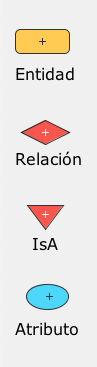
\includegraphics[width=0.15\textwidth]{img/barra_lateral.png}
    \caption{Barra lateral para añadir elementos}
\end{figure}
Dentro del área de diseño se ha añadido una barra lateral que permite agregar nuevos elementos al diagrama. De esta forma se consigue que el usuario pueda crear elementos nuevos de una forma más intuitiva que haciendo clic derecho sobre el panel de diagrama. A continuación se detallan las principales características de este panel.

\begin{itemize}
    \item Permite al usuario añadir cuatro tipos de elementos: entidades, relaciones, relaciones ISA y atributos.\\
    
    Los botones de añadir entidad y añadir relación muestran el cuadro de diálogo correspondiente, en el que se permite insertar el nombre y las características del elemento.\\
    
    El botón ISA, al no necesitar nombre ni configuración, inserta directamente la relación en el diagrama.\\
    
    El botón atributo permite seleccionar mediante un menú desplegable a qué entidad o relación pertenece el atributo, también se le pide al usuario el nombre y las características del atributo.
    \item Los elementos se insertan automáticamente en el diagrama. Al no haber hecho clic derecho el usuario en ningún punto del diagrama, el programa no dispone de una posición de referencia en la que el elemento debe ser insertado. Por ello el programa genera unas coordenadas automáticamente.
    \begin{itemize}
        \item Las \textbf{entidades} y \textbf{relaciones} nuevas empiezan a colocarse a partir de la esquina superior izquierda del panel. Los elementos sucesivos se colocan a la derecha del anterior, dejando un pequeño margen.\\
        
        El programa dispone del tamaño exacto que tiene el panel de diseño en cada momento, por tanto cuando se intenta insertar un elemento a la derecha del anterior, pero quedando fuera del diagrama, el programa lo genera en una línea inferior.
        \begin{figure}[H]
            \centering
            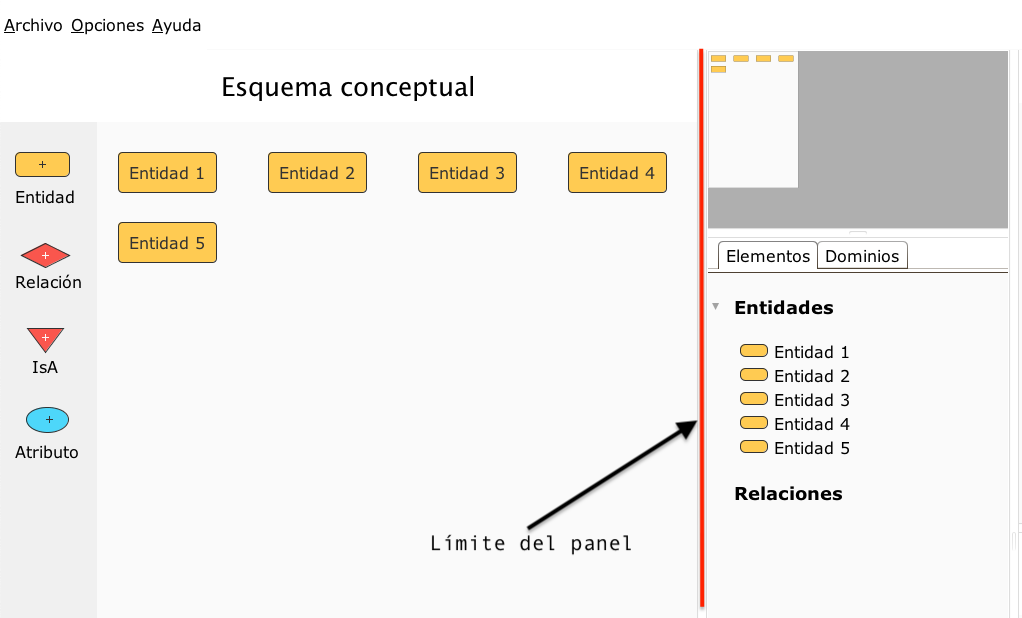
\includegraphics[width=0.8\textwidth]{img/limitepanel.png}
            \caption{Colocación de nuevos elementos}
        \end{figure}
        \item Los \textbf{atributos} siguen un comportamiento distinto debido a que dependen de la relación o entidad a la que pertenezcan. Los nuevos atributos se generan creando círculos concéntricos alrededor del elemento al que pertenecen, a diferencia de la versión anterior en la que simplemente se generaban a la derecha del elemento.\\
        
        Para realizar el cálculo de las coordenadas se ha creado una función con la ayuda de la función "sin" de la librería Math \cite{math}, que tiene en cuenta el número de atributos del elemento, el ancho del elemento y la distancia a los márgenes del diagrama (evitando que se generen nuevos atributos en posiciones negativas, obligando al usuario a desplazar el diagrama).\\
        
        \begin{lstlisting}[
                   xleftmargin = -3.4cm,language=java]
        p.setLocation(
				Math.round(ancho*Math.sin(offset/(Math.PI/constant))+p.getX()), 
				Math.round(alto*Math.sin(offset/(Math.PI/constant)-(Math.PI/2))+p.getY())
				);
        \end{lstlisting}
    \end{itemize}
\end{itemize}
\subsection{Paneles de texto}
La forma en la que se presentan los códigos generados ha cambiado radicalmente, como se ha comentado anteriormente se ha dividido en dos paneles (modelo lógico y modelo físico). A continuación se describen en detalle todos los cambios que han sufrido.
\begin{itemize}
    \item Se han eliminado los botones de validar modelo y de limpiar área de texto.
    \item La validación del modelo ahora se hace de forma automática cuando el usuario pulsa el botón de generar código (tanto para el modelo lógico como para el modelo físico).
   \item La validación ahora solo muestra mensajes cuando existen errores o alertas en el diagrama. Anteriormente informaba de todas las comprobaciones realizadas, fueran correctas o no.
   \item Ha desaparecido el botón de limpiar área y en su lugar los cuadros de texto son completamente editables, dando libertad al usuario para modificar o añadir cualquier texto que desee.
   \item Los paneles han sufrido también un gran cambio en el aspecto visual. Están construidos mediante una clase "ReportPanel" que hereda de JTextPane. La clase modifica el panel pana que muestre contenido HTML mediante la función.\\
   \begin{lstlisting}[backgroundcolor = \color{white},
                   xleftmargin = 2cm,language=java,basicstyle=\medium]
        setContentType("text/html");\end{lstlisting}
        

   El texto ahora se interpreta como código HTML y se representa como tal, lo que amplía enormemente las posibilidades de diseño. Se ha añadido en el código una sección css con los estilos del panel. Los estilos son generados teniendo en cuenta el tema seleccionado por el usuario y modifican varios aspectos como:
   \begin{itemize}
       \item Párrafos.
       \item Títulos.
       \item Listas.
       \item Divisores.
       \item Color de fondo.
       \item Fuente y color de las letras.
   \end{itemize}
   \begin{figure}[H]
            \centering
            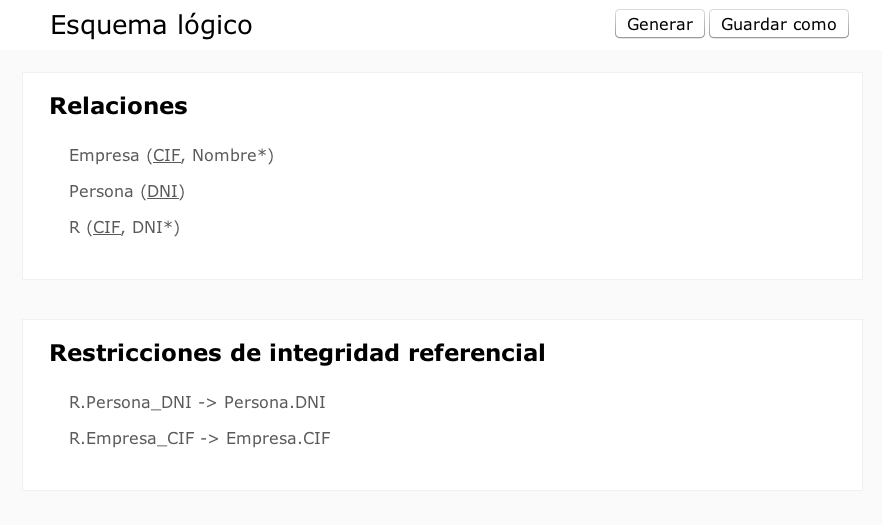
\includegraphics[width=0.8\textwidth]{img/ejemploreport.png}
            \caption{Ejemplo de modelo relacional.}
    \end{figure}
    Como se puede observar se ha optado por un diseño que divide en tarjetas las distintas secciones del código. Los mensajes de error y de aviso aparecen en distintos colores y se ubican siempre en la parte superior.
    \begin{figure}[H]
            \centering
            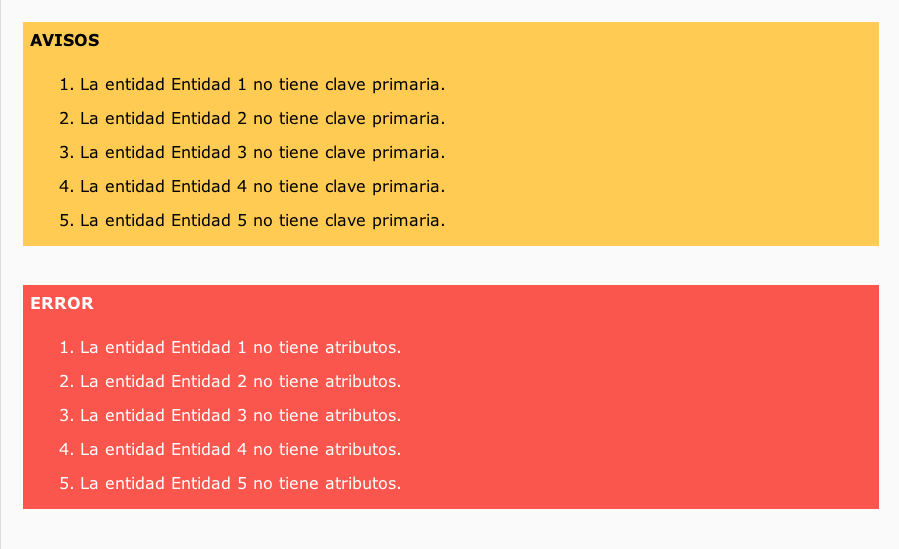
\includegraphics[width=0.8\textwidth]{img/ejemploreport2.png}
            \caption{Ejemplo de mensajes de aviso y error.}
    \end{figure}
\end{itemize}
\subsection{Perspectivas}
Se ha implementado la posibilidad de elegir distintas perspectivas en las que se colocan los paneles en función de las necesidades del usuario. En la parte superior derecha de la aplicación aparece un menú de selección de perspectiva. Los iconos son generados mediante la librería Graphics2D \cite{g2d} y se adaptan a los colores del tema. Funcionan como "Botones de Radio", es decir que solo se permite tener seleccionada una de las perspectivas.\\
\begin{figure}[H]
            \centering
            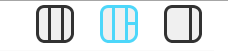
\includegraphics[width=0.5\textwidth]{img/perspectivas.png}
            \caption{Menú de selección de perspectiva.}
\end{figure}

Se han desarrollado tres perspectivas:
\begin{itemize}
    \item \textbf{Código}: Divide la pantalla en tres paneles: panel de información / dominios, panel de esquema lógico y panel de esquema físico. Está pensado para permitir al usuario centrarse en la edición de códigos. Mantiene el panel de información / dominios para servir de referencia del diagrama dibujado.
    \item \textbf{Completo}: Integra todos los paneles posibles y sirve para que el usuario tenga una visión global de todo el trabajo.
    \item \textbf{Diseño}: Muestra el panel de diseño, la barra de añadir elementos y el panel de información / dominios. Con él se centra la atención en el diseño del modelo entidad relación dando todo el espacio de la pantalla para ello.
\end{itemize}

\subsection{Cambios en el panel de diseño}
El panel de diseño también ha sufrido algunos cambios desde la versión anterior, aunque en general el panel sigue teniendo un comportamiento similar y los cambios producidos aquí han sido de poco impacto.

\begin{itemize}
    \item Se ha cambiado el aspecto de los elementos, añadiendo colores, resaltando los bordes cuando el elemento está seleccionado, cambiando la fuente de texto, y redondeando los bordes de las entidades.
    \item Se ha acercado el zoom por defecto tanto en el panel principal como en en la miniatura, y se ha corregido la orientación del scroll para hacer zoom (funcionaba al revés de lo intuitivo).
    \item Se han añadido flechas en las relaciones que lo requieren y también se han implementado las dobles líneas para las relaciones de participación total.
\end{itemize}
\subsection{Cambios en los cuadros de diálogo}
DBCase dispone de cuadros de diálogo para realizar tareas como crear una relación, editar la cardinalidad de una entidad o guardar el proyecto en un archivo.\\

En ésta versión se han modificado todos los cuadros de la siguiente manera.
\begin{itemize}
    \item Se han adaptado todos los elementos para adaptarlos a los temas elegidos por el usuario.
    \item Se han eliminado los iconos que acompañaban a muchos de los cuadros y se ha simplificado su diseño. Se ha aumentado el tamaño de los cuadros de introducción de texto.
\end{itemize}
\subsection{Menú}
El menú de opciones también ha sufrido algunos pequeños cambios.
\begin{itemize}
    \item Se han quitado los iconos que acompañaban a algunas de las opciones del menú, se ha aumentado el tamaño de letra y se ha conseguido que el menú se adapte al tema vigente. Para ello ha sido necesario crear una clase que herede de JMenuBar \cite{menu} y que modifique uno a uno los componentes necesarios.
    \item En el menú de opciones se han quitado las opciones de ocultar el panel de sucesos (el panel ya no existe), y seleccionar el gestor de Base de Datos actual (Esta opción se ha desplazado al panel de esquema físico).\\
    
    En su lugar se han añadido un menú desplegable para seleccionar el tema de entre todos los disponibles en la carpeta "themes", y una opción para mostrar o no los atributos posiblemente nulos.
    
    \item Se ha actualizado el texto de "Acerca de DBCASE".
\end{itemize}
\subsection{Archivo abierto}
En la versión anterior existía un panel al pie de la aplicación que indicaba el directorio de trabajo actual, con la información del archivo temporal que se estaba usando para guardar los cambios en la aplicación. Esta información no era demasiado relevante para el usuario, y sería más útil indicar cual es el archivo abierto por el usuario.\\

También existía en la barra de menús un botón que funcionaba como un semáforo de cambios (adoptaba el color verde cuando todos los cambios estaban guardados y el color rojo cuando existían cambios en el archivo temporal sin guardar en el archivo final). Finalmente este botón se ha quitado.\\

Como solución se ha pensado indicar en la cabecera del programa cual es el archivo (xml) abierto por el usuario (en caso de que no haya creado un archivo nuevo). Si existen cambios en el programa sin guardar, el nombre del archivo viene seguido de un asterisco (*).\\

De esta forma se han unificado y mejorado ambas funcionalidades en un espacio más reducido.

\subsection{Logotipo}
\begin{figure}[H]
    \centering
    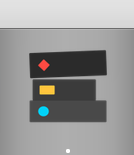
\includegraphics[width=0.3\textwidth]{img/logoMac.png}
    \caption{DBCASE en el dock de MacOS}
\end{figure}
Se ha diseñado un nuevo logotipo para la aplicación. El diseño está inspirado en el stack con el que se suelen representar las bases de datos. Se ha buscado darle aspecto de letra E mayúscula, ya que es la última letra del nombre del programa, y se han incluido una representación de los tres elementos principales del modelo entidad relación (atributos, entidades y relaciones).\\

El logotipo aparece como icono de la aplicación tanto en sistemas operativo Windows como MacOS.

%%%%%%%%%%%%%%%%
\section{Funcionalidad}
Los cambios a nivel de funcionalidad se han centrado principalmente en las traducciones desde el esquema conceptual a los esquemas lógico y físico. Se han corregido algunos errores arrastrados desde la versión anterior, y se han implementado nuevas traducciones, mejorando sobre todo el esquema lógico.

\subsection{Esquema lógico}

La traducción del diagrama entidad relación al modelo relacional ha sufrido grandes mejoras en esta versión.
\begin{itemize}
    \item Se ha depurado la traducción al modelo relacional, corrigiendo errores arrastrados desde la anterior versión.
    \item Se han añadido varias secciones nuevas al esquema lógico.
    \begin{itemize}
        \item \textbf{Restricciones de integridad referencial}: En esta sección aparecen descritas de forma esquemática las restricciones de integridad referencial \cite{rir} generadas a partir del diagrama entidad relación.
        \item \textbf{Restricciones perdidas}: Aquí aparecen todas las restricciones que pueden generarse a raíz del diagrama, pero que no son representadas en el modelo relacional.
        \begin{itemize}
            \item \textbf{Cardinalidad}: indica las restricciones que se pierden con respecto a la cardinalidad de las relaciones, por ejemplo para una cardinalidad de 1 a 23, indica que se ha perdido la cardinalidad máxima de 23 en la entidad.
            \item \textbf{Restricciones de tabla}: muestra las restricciones de tabla introducidas manualmente por el usuario, así como algunas restricciones asociadas a los atributos (por ejemplo que el atributo sea de tipo unique).
            \item \textbf{Claves candidatas}: informa de los atributos que funcionan como clave candidata de una determinada tabla.
        \end{itemize}
    \end{itemize}
\end{itemize}
\subsection{Exportación de códigos}
Con respecto a la exportación de los códigos se han implementado las siguientes mejoras.

\begin{itemize}
    \item Se han implementado dos botones de exportación: uno para el esquema lógico y otro para el esquema físico. De esta forma se pueden guardar los códigos de forma independiente. El esquema lógico puede ser guardado en formato .txt, mientras que el esquema físico puede ser guardado en formato .sql y en formato .txt.
    \item Se ha añadido la capacidad de guardar el texto modificado escrito por el usuario, de forma que al guardar el texto se guarda con las modificaciones existentes.
    \item Esto también ocurre a la hora de ejecutar el código sql del esquema físico. El código ejecutado es el código con las modificaciones del usuario.
    \item Para hacer posible el guardado y la ejecución de los códigos modificados, y dado que los paneles de texto funcionan con el formato HTML, ha sido necesaria la implementación de un sistema de traducción de texto HTML a texto plano.
\end{itemize}
\subsection{Atributos posiblemente nulos}
\begin{figure}[H]
    \centering
    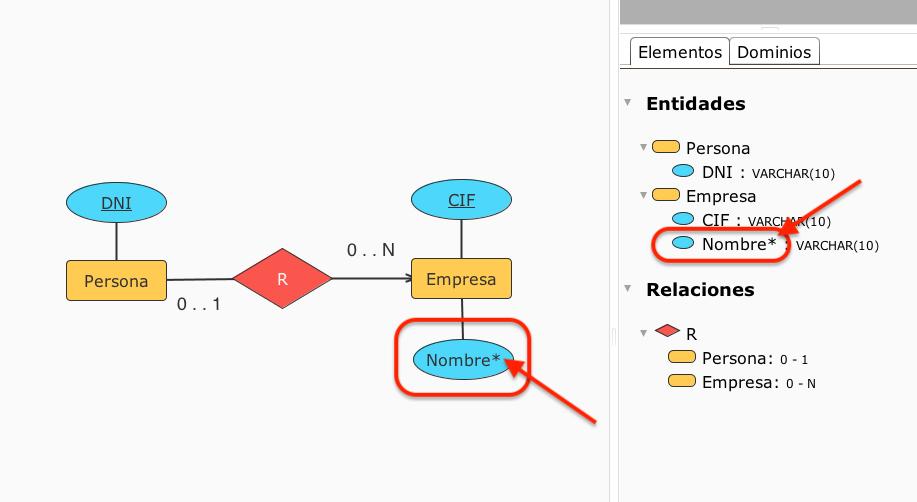
\includegraphics[width=\textwidth]{img/nulls.png}
    \caption{Representación de atributo posiblemente nulo.}
\end{figure}
Se ha implementado la capacidad de identificar los atributos posiblemente nulos. Si la opción está activada en el menú, los atributos que cumplan el requisito se mostrarán tanto en el panel de diseño, como en el panel de elementos y en el modelo relacional con un asterisco (*) al final del nombre del mismo.
\subsection{Desplazamiento del diagrama}
Se a añadido la opción de desplazar el diagrama en los ejes x e y manteniendo pulsada la barra espaciadora y arrastrando el panel. De esta forma se añade otra opción más a parte de la miniatura del diagrama para realizar el desplazamiento.
\\

\begin{lstlisting}[xleftmargin = 2cm,language=java]
//Funcion que cambia el modo de uso del panel
public void toggleDragMode(boolean b) {
		if(b==mouseMode) return;
		if(!mouseMode) {
		//cambia el panel a modo desplazamiento
			creaGraphMouse();
			//Se anade el plugin de desplazamiento
			graphMouse.add(translating);
			graphMouse.setMode(ModalGraphMouse.Mode.TRANSFORMING);
			vv.setGraphMouse(graphMouse);
		}else {//cambia el panel a modo edición
			creaGraphMouse();
			//Se anade el plugin de edicion
			graphMouse.add(picking);
			graphMouse.setMode(ModalGraphMouse.Mode.PICKING);
			vv.setGraphMouse(graphMouse);
		}
		mouseMode = !mouseMode;
	}
\end{lstlisting}

El panel de diseño esta implementado usando la clase VisualizationViewer \cite{vv} (objeto vv en el ejemplo), disponible el la librería de Jung \cite{jung}. El funcionamiento del ratón viene dado por el objeto GraphMouse, cuyo funcionamiento depende del plugin que posea en cada caso.
\subsection{Guardado de configuraciones}
El archivo dbcase.config almacena algunas de las configuraciones del programa (como el lenguaje o el último archivo abierto), de forma que la próxima vez que el usuario inicie la aplicación estas configuraciones son recordadas. Ahora este archivo también almacena el último tema escogido por el usuario y la última perspectiva usada.

%%%%%%%%%%%%%%%%
\section{Código}
\begin{comment}
- Estructura de paneles
- Carpeta projects
- Implementacion con git
\end{comment}